\documentclass[9pt]{beamer}    % chane text size from here [9pt], or [8pt]
%
% Choose how your presentation looks.
%
% For more themes, color themes and font themes, see:
% http://deic.uab.es/~iblanes/beamer_gallery/index_by_theme.html
%
\mode<presentation>
{
  \usetheme{Madrid}      % or try Darmstadt, Madrid, Warsaw, ...
  \usecolortheme{beaver} % or try albatross, beaver, crane, ...
  \usefonttheme{professionalfonts}  % or try serif, structurebold, ...
  \setbeamertemplate{navigation symbols}{}
  \setbeamertemplate{caption}[numbered]
} 
\setbeamertemplate{bibliography item}[text]  % Command to show reference numbered 
\usepackage[english]{babel}
\usepackage[utf8x]{inputenc}
%\usepackage{wrapfig}
\usepackage{graphicx}



\title[UCDavis]{Neutrino Event Generator:  GENIE - tutorials}
\author{Jaydip Singh}
\institute[] % (optional)
{%University of Lucknow, India \\
 Postdoc at Department of Physics and Astronomy, UC Davis\\
 %for the DUNE collaboration.
%Dr. Thomas R. Junk\\
%FNAL, Batavia, USA \\
 %Dr. Jyotsna Singh\\

}\date{21/01/2020}
\date[]{April 22-26, 2024}

\begin{document}

\begin{frame}
  \titlepage\centering\textbf{ Understanding The Universe Through Neutrinos} \\
  % \textsf{FERMILAB-SLIDES-20-097-LBNF}
  \begin{figure}[!htb]
   \begin{minipage}{0.30\textwidth}
     \centering
     
\includegraphics[width=.60\linewidth]{UC-Davis-Logo.png}
     
   \end{minipage}\hfill
   \begin{minipage}{0.30\textwidth}
     \centering
     
\includegraphics[width=.45\linewidth]{icts_logo.jpeg}
    
   \end{minipage}
\end{figure}
\end{frame}


\begin{frame}{Outlines : }
\begin{itemize}
 \item Can we do better than SAND detector to understand the systematics due to nuclear effect ?

 \item What is the neutrino energy range that we can detect at ANNIE phase-II and Phase-III ?

 \item Can we measure $Q^{2}$ at 2.5 GeV neutrino beam energy at ANNIE data ?

 \item Can we understand missing hadrons energy at 2.5 GeV neutrino beam energy with ANNIE phase II or Phase III data ?

\end{itemize}

\end{frame}




\begin{frame}{Neutrino-Nucleus Interactions}
\begin{itemize}
 \item \small{A neutrino interacts via charged current and neutral current interactions.}
\end{itemize}

\begin{figure}[!htb]
   \begin{minipage}{0.48\textwidth}
     \centering
     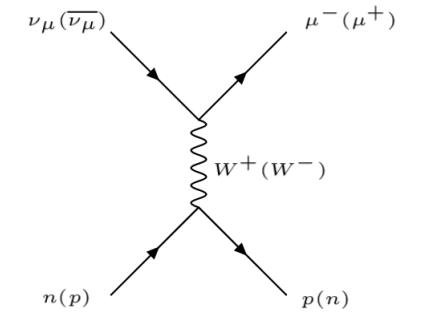
\includegraphics[width=.62\linewidth]{ccfig.jpg}

   \end{minipage}\hfill
   \begin{minipage}{0.48\textwidth}
     \centering
     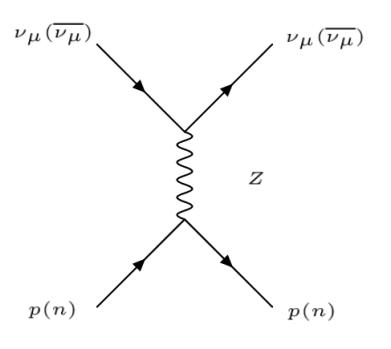
\includegraphics[width=.62\linewidth]{ncfig.jpg}

   \end{minipage}
   \end{figure}
\begin{itemize}
 \item \small{Various energy dependent neutrino interaction processes}
\end{itemize}

\begin{figure}
 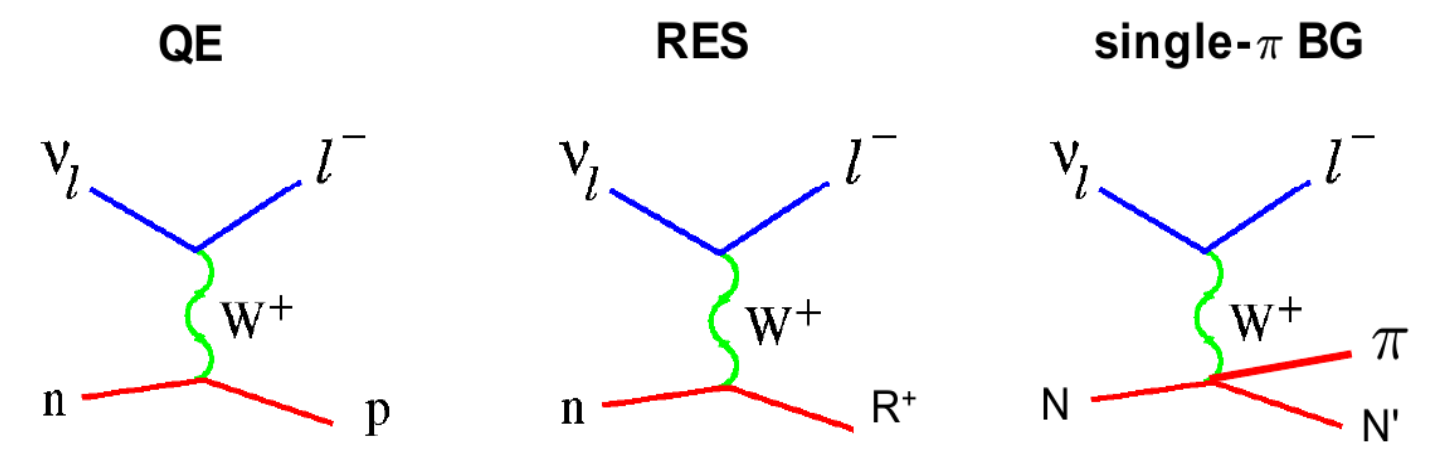
\includegraphics[scale=.15]{allprocess.jpg}
 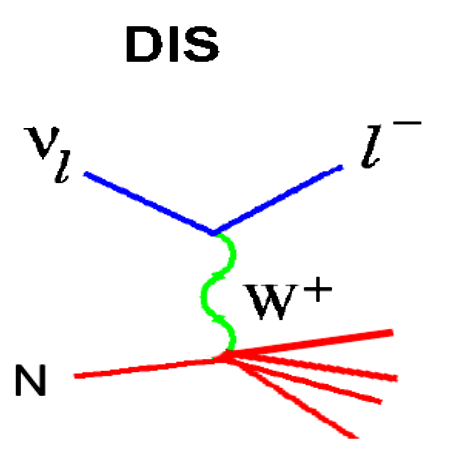
\includegraphics[scale=.15]{dis.jpg}
\end{figure}
\end{frame}


\begin{frame}{Nuclei as Targets}
 \begin{itemize}
 \begin{small}
  \item To increase neutrino interaction rates: experiments use heavy nuclear targets with high atomic mass numbers like Ar(A=40), C(A=6), Ca(A=40).
  \item Heavy nuclear targets gives a boost to the event statistics in turn reducing the statistical uncertainties but at the same gives rise to the systematic uncertainties which are ultimately required to be tuned.
  \end{small}
 \end{itemize}
\begin{figure}
 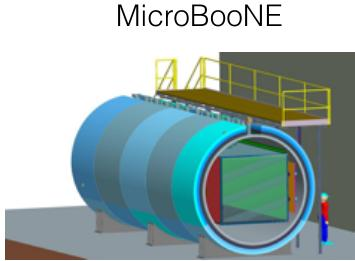
\includegraphics[scale=.28]{p1.jpg}
 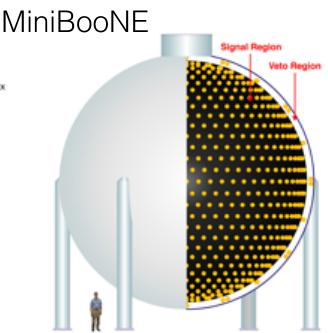
\includegraphics[scale=.28]{p2.jpg}
 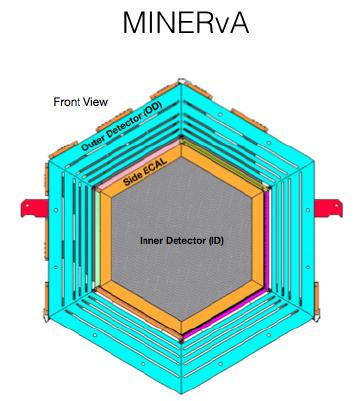
\includegraphics[scale=.28]{p3.jpg}
 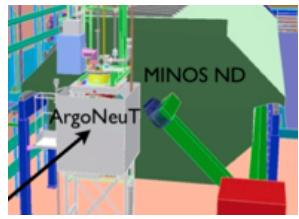
\includegraphics[scale=.30]{p4.jpg}
 \end{figure}
\end{frame}


\begin{frame}{Hydrogen Target}
 \begin{itemize}
 \begin{small}
  \item Control sample free from nuclear effects to calibrate (anti)neutrino energy scale.
  \item Direct constraints on nuclear effects required to reduce systematics from nuclear targets.
  \item Straw Tube Tracker designed for a control of $\nu$ - target(s), proposed to build at ND hall.
  \item Separation from excellent vertex, angular and timing resolutions\footnotemark.
  \item Thin targets replaceable during data taking  CH$_{2}$, C, Ca, Fe, Pb, etc.
  \end{small}
 \end{itemize}
\begin{figure}
 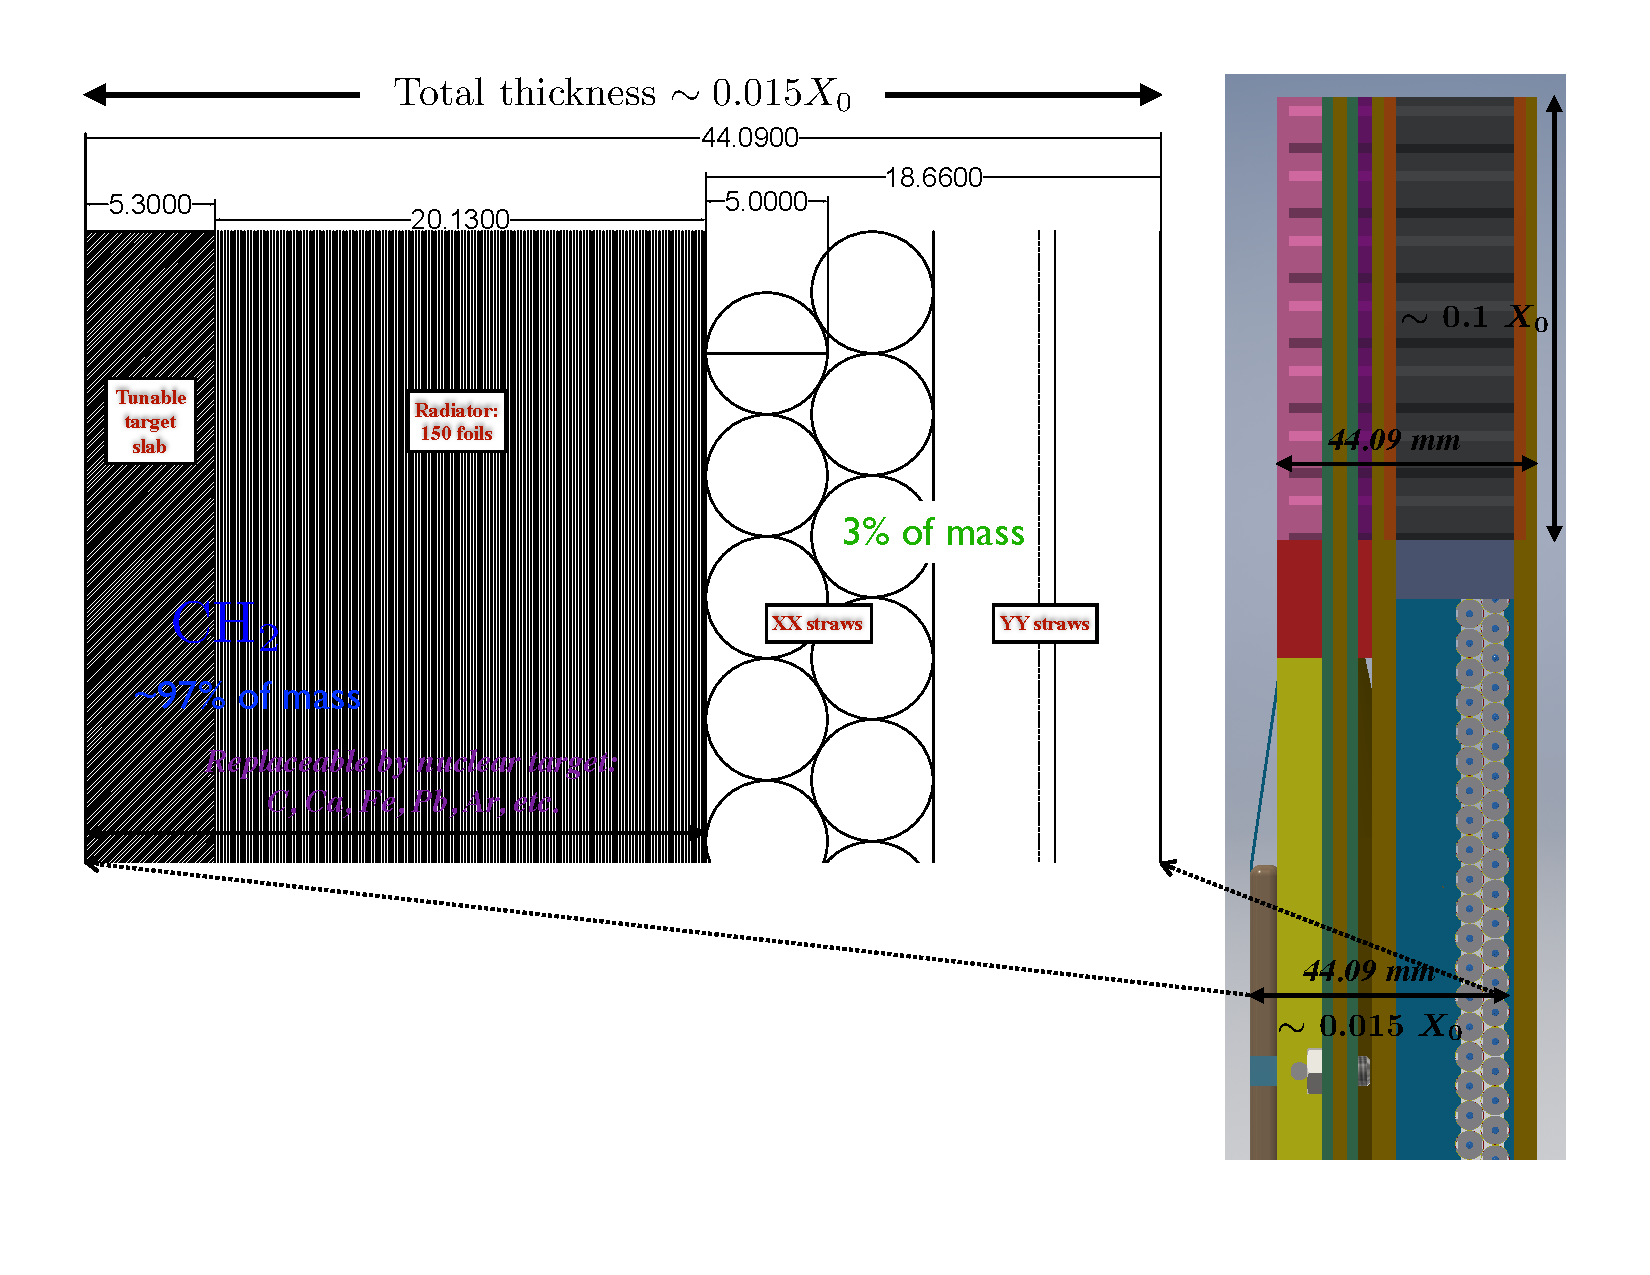
\includegraphics[scale=.20]{CompactSTT.pdf}
 \end{figure}
 \footnotetext[7]{ R. Petti (South Carolina ), (\href{https://indico.phys.vt.edu/event/44/contributions/884/attachments/758/1011/NDNN21_Petti.pdf}{\beamergotobutton{NDNN(nustec2021)}}) }
\end{frame}


 \begin{frame}{Nuclear Effects}
 \begin{minipage}{0.6\textwidth}\raggedright
\begin{small}
 \begin{itemize}
  \item \textbf{Initial State Interactions}
  \begin{itemize}
   \item Nuclear Binding
   \item Fermi motion
   \item Pauli blocking
  \end{itemize}
 \end{itemize}

 \begin{itemize}
  \item \textbf{Final State Interactions}
  \begin{itemize}
  \item absorption of outgoing particles
   \item rescattering, charge exchange
   \item production of new particles
  \end{itemize}
 \end{itemize}
 \begin{itemize}
  \item A model must include realistic description of nuclear effects including both ISI and FSI
 \end{itemize}

\end{small}
\end{minipage}
\hfill%
  \noindent\begin{minipage}{0.38\textwidth}% adapt widths of minipages to your needs
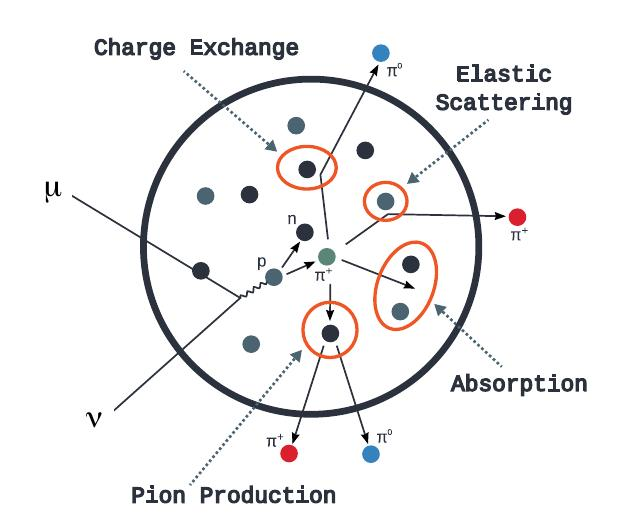
\includegraphics[scale=.30]{nuceff2.jpg}
\end{minipage}%
\end{frame}




\begin{frame}{Uncertainties in the $\nu$-nucleus cross-section}
\begin{itemize}
 \item Two main reasons:
 \begin{itemize}
  \item poor knowledge of neutrino flux
  \item recent cross section measurements have been performed on nuclear targets
 \end{itemize}
 \item Neutrino experiments measure a convolution of energy dependent neutrino flux $\bigotimes$ energy dependent cross-section $\bigotimes$ energy dependent nuclear effects.
 \item Interacting neutrino energy is evaluated based on kinematics of particles in the final state, taking into account detector acceptance.

\end{itemize}
\end{frame}



\begin{frame}{Calorimetric technique}
\begin{itemize}
 \item Applying the calorimetric approach i.e. summing up all the outgoing particles, $E_{\nu}^{Calor}$ (reconstructed neutrino energy), can be calculated as-
\begin{equation}
 E_{\nu}^{Calor} = E_{lep}+ \sum \limits_{i} T_{i}^{nuc} + \epsilon_{nuc} + \sum \limits_{m} E_{m}
\end{equation}
\item where $E_{lep}$ is the outgoing final state charged lepton's energy, $T_{i}^{nuc}$ is the kinetic energies of the outgoing nucleons(i.e. the protons and/or neutrons), their corresponding separation energies represented as $\epsilon_{nuc}$ and total energy of any other particle produced represented as $E_{m}$.
\item We can also write Equation(1) as- $E_{\nu}^{Calor} = E_{lep}+E_{had}$, where,
\begin{equation}
 E_{had} = \sum \limits_{i} T_{i}^{nuc} + \epsilon_{nuc} + \sum \limits_{m} E_{m}
\end{equation}
\end{itemize}
\end{frame}



\begin{frame}{Kinematics technique}
\begin{itemize}
 \item For incoming neutrino with an energy $<$ 1 GeV, CCQE interaction is the dominant interaction mode.
 \item The two-body  kinematics of this interaction offers a simplified calculation of neutrino energy by using the kinematics of the outgoing lepton only i.e. the angle and energy of the outgoing muon.

\begin{equation}
 E_{rec}^{\nu} = \frac{2(M - E_{b})E_{\mu} - (E_{b}^{2} - 2ME_{b} + m_ {\mu}^{2} + \Delta M^{2})}{2(M - E_{b}- E_{\mu} + |\vec{p_{\mu}}|cos \theta_{\mu})}
\end{equation}
\item Here $E_{\mu}$, $m_{\mu}$, $p_{\mu}$ is the energy, mass and momentum of the outgoing muon and $\theta_{\mu}$ is the angle between the direction of outgoing muon and incoming neutrino. M is the mass and $E_{b}$ is the binding energy of the struck neutron.
\item $\Delta M^{2} = M_{n}^{2} - M_{p}^{2}$ .

\end{itemize}
\end{frame}

\begin{frame}{$Q^{2}$ Estimation}
 \begin{itemize}
  \item $Q^{2}$ is calculated as-
  \begin{equation}
   Q^{2} = 2E_{rec}^{\nu}(E_{\mu}-p_{\mu}cos \theta_{\mu}) - M^{2}_{\mu}
  \end{equation}
 where $M_{\mu}$, $p_{\mu}$, $E_{\mu}$ and $\theta_{\mu}$ are the mass, momentum, energy and angle of the outgoing muon.
 \end{itemize}

\begin{figure}
 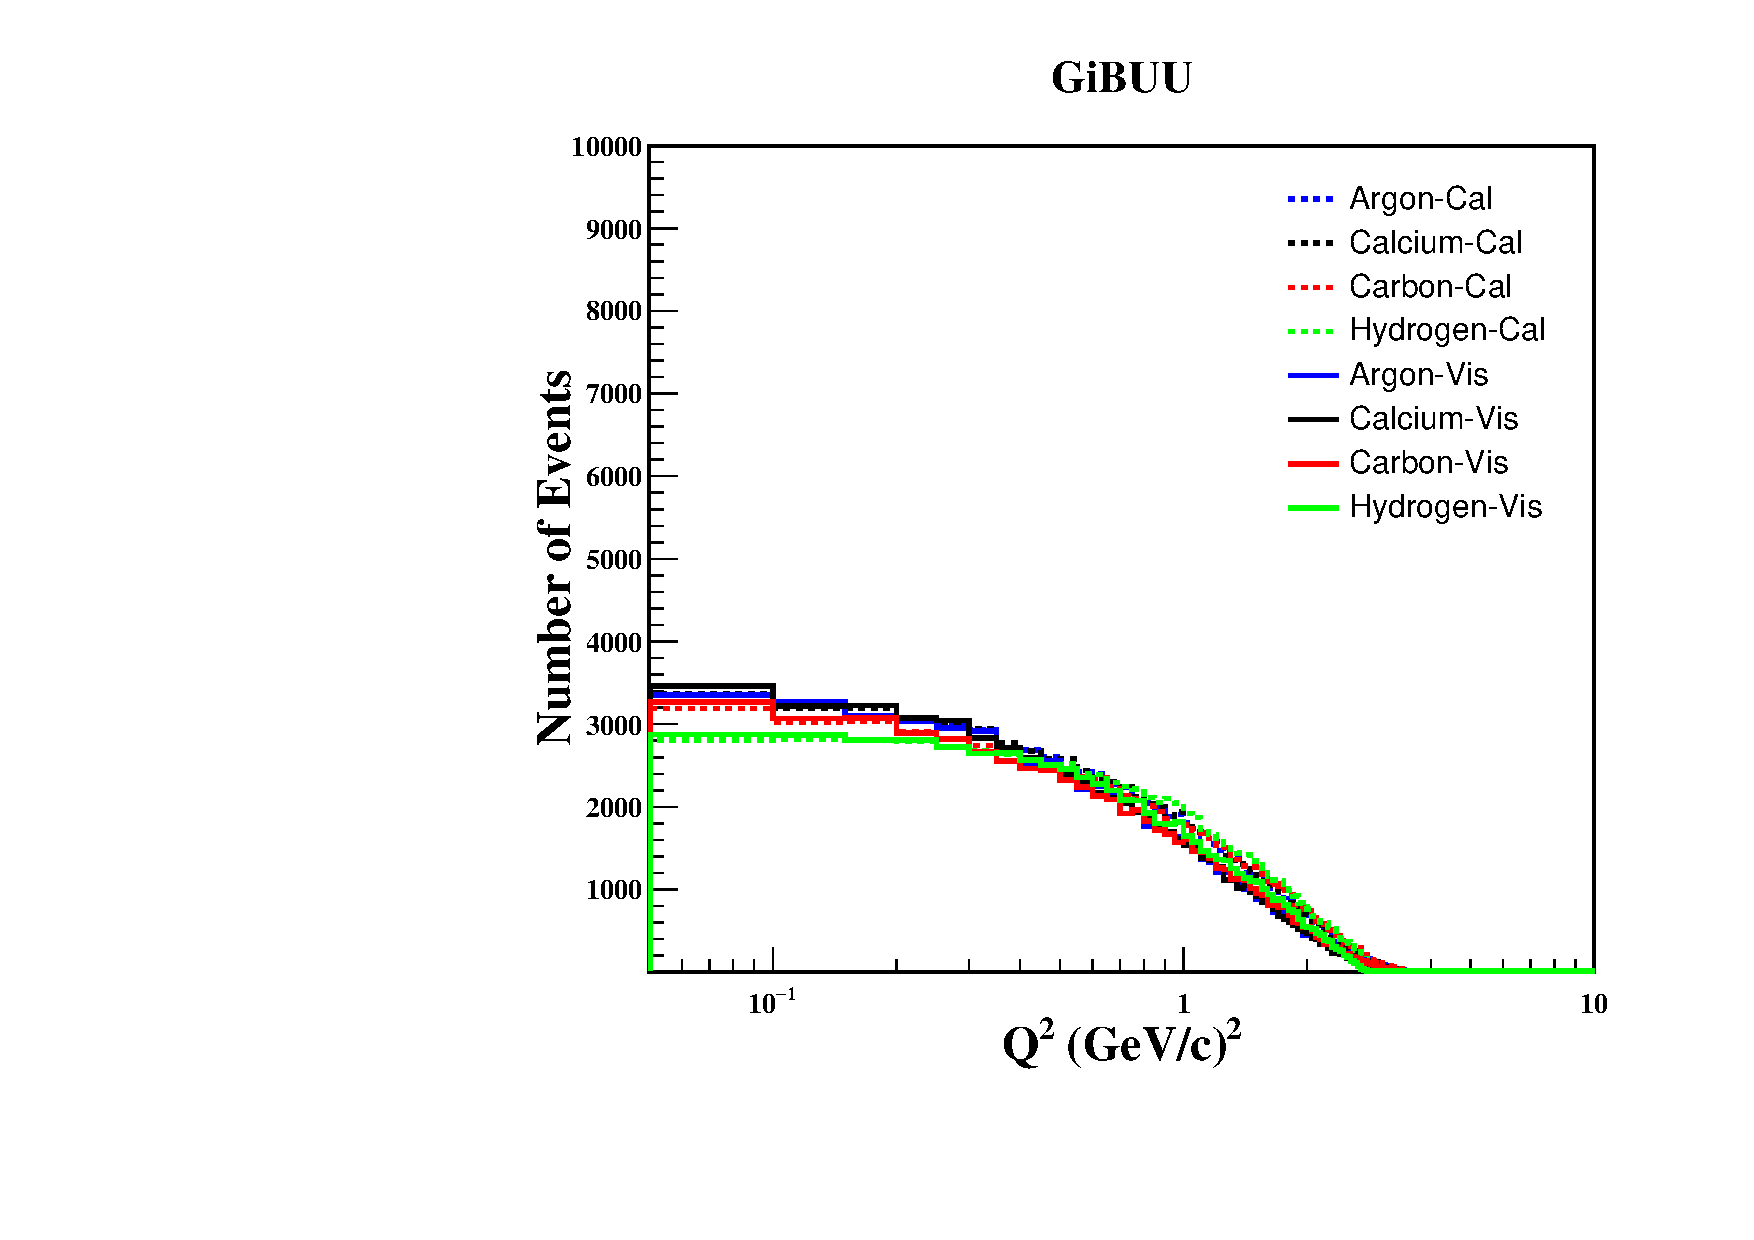
\includegraphics[scale=0.30]{AllTargetsQ2norm}
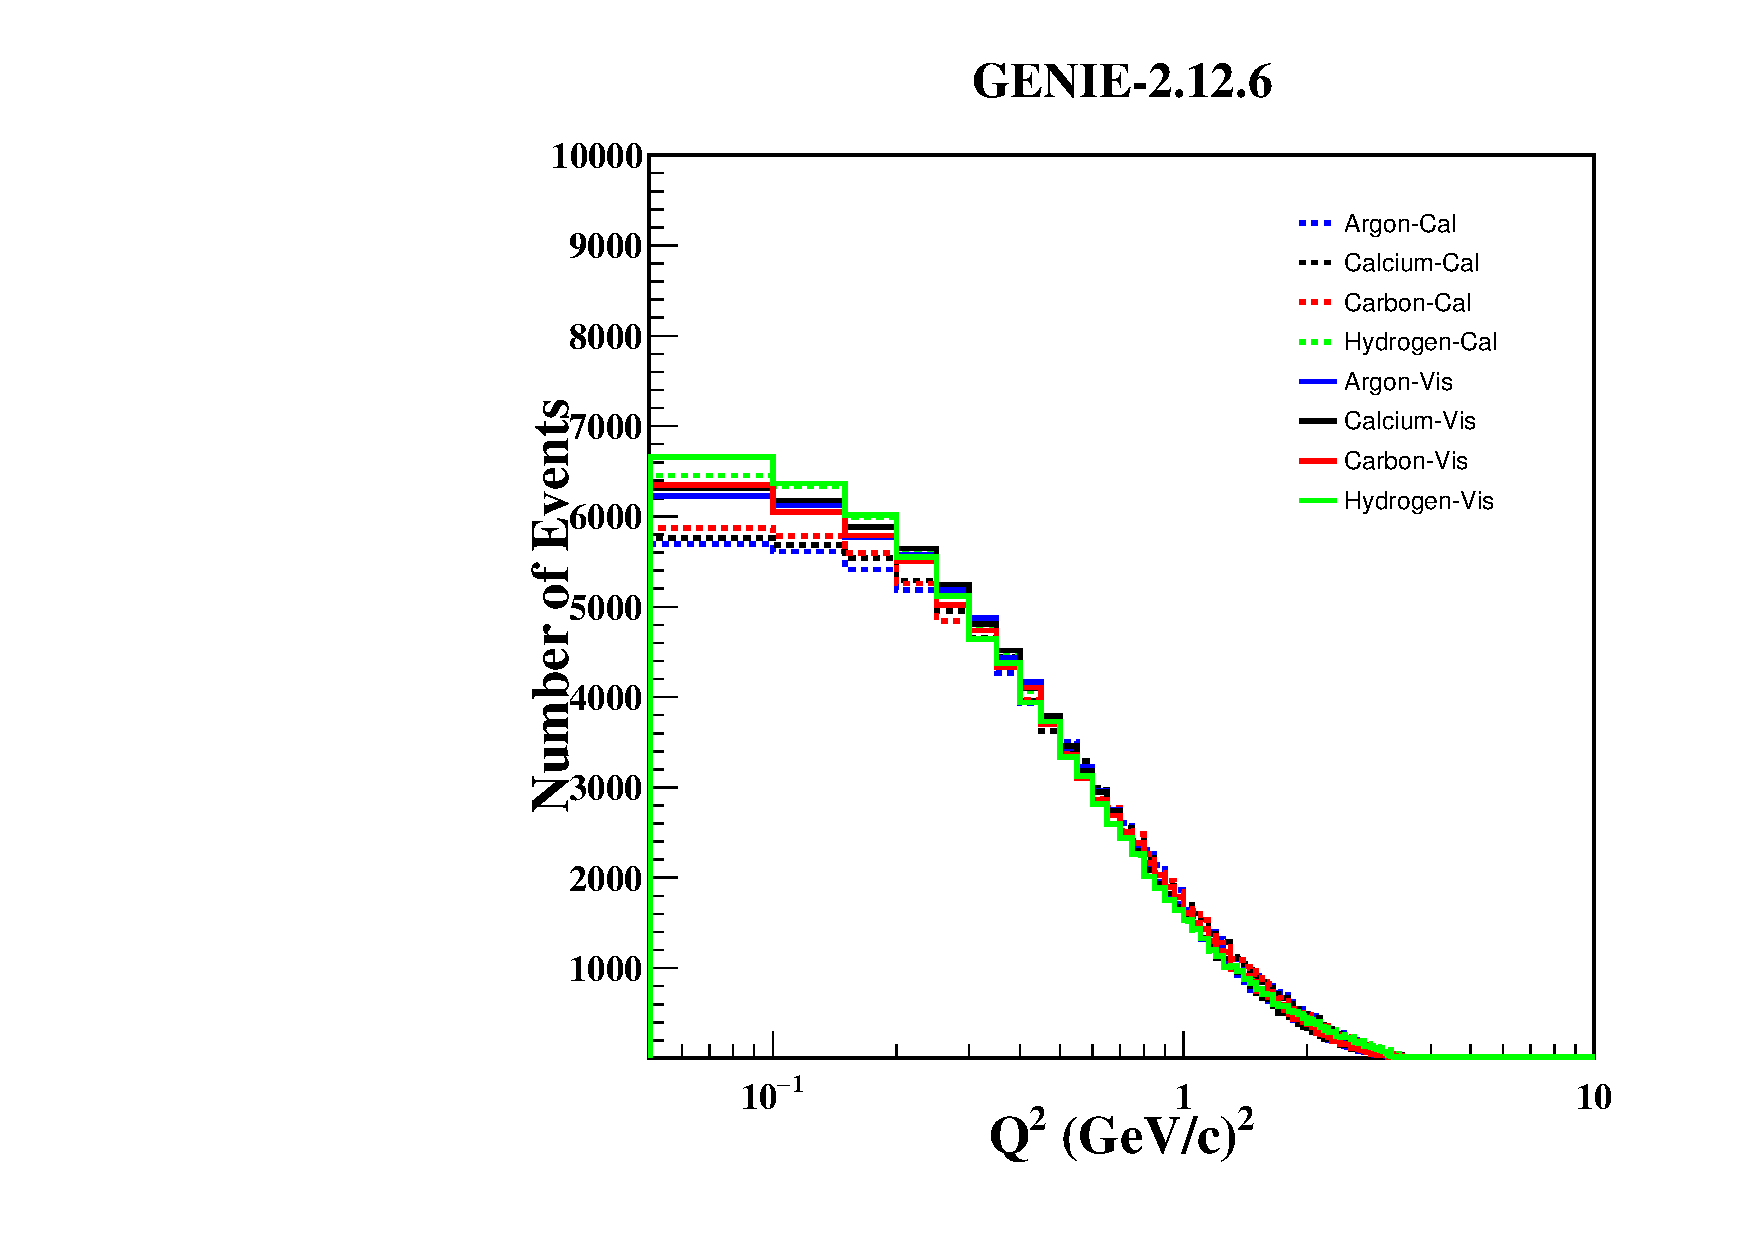
\includegraphics[scale=0.27]{AllTargetQ25GeVGenie}
\end{figure}
\end{frame}

\begin{frame}{Missing Hadrons Analysis}
 \begin{itemize}
\item \textbf{RNeutNu}  = KE-Neutron/EnuTrue \newline This ratio defines the fraction of kinetic energy of neutrons with respect to the true neutrino energy.
\item \textbf{RNHadNu} = KE-NeutralHadrons/EnuTrue \newline This ratio defines kinetic energy of neutral hadrons with respect to the true neutrino energy.
\end{itemize}

\begin{figure}
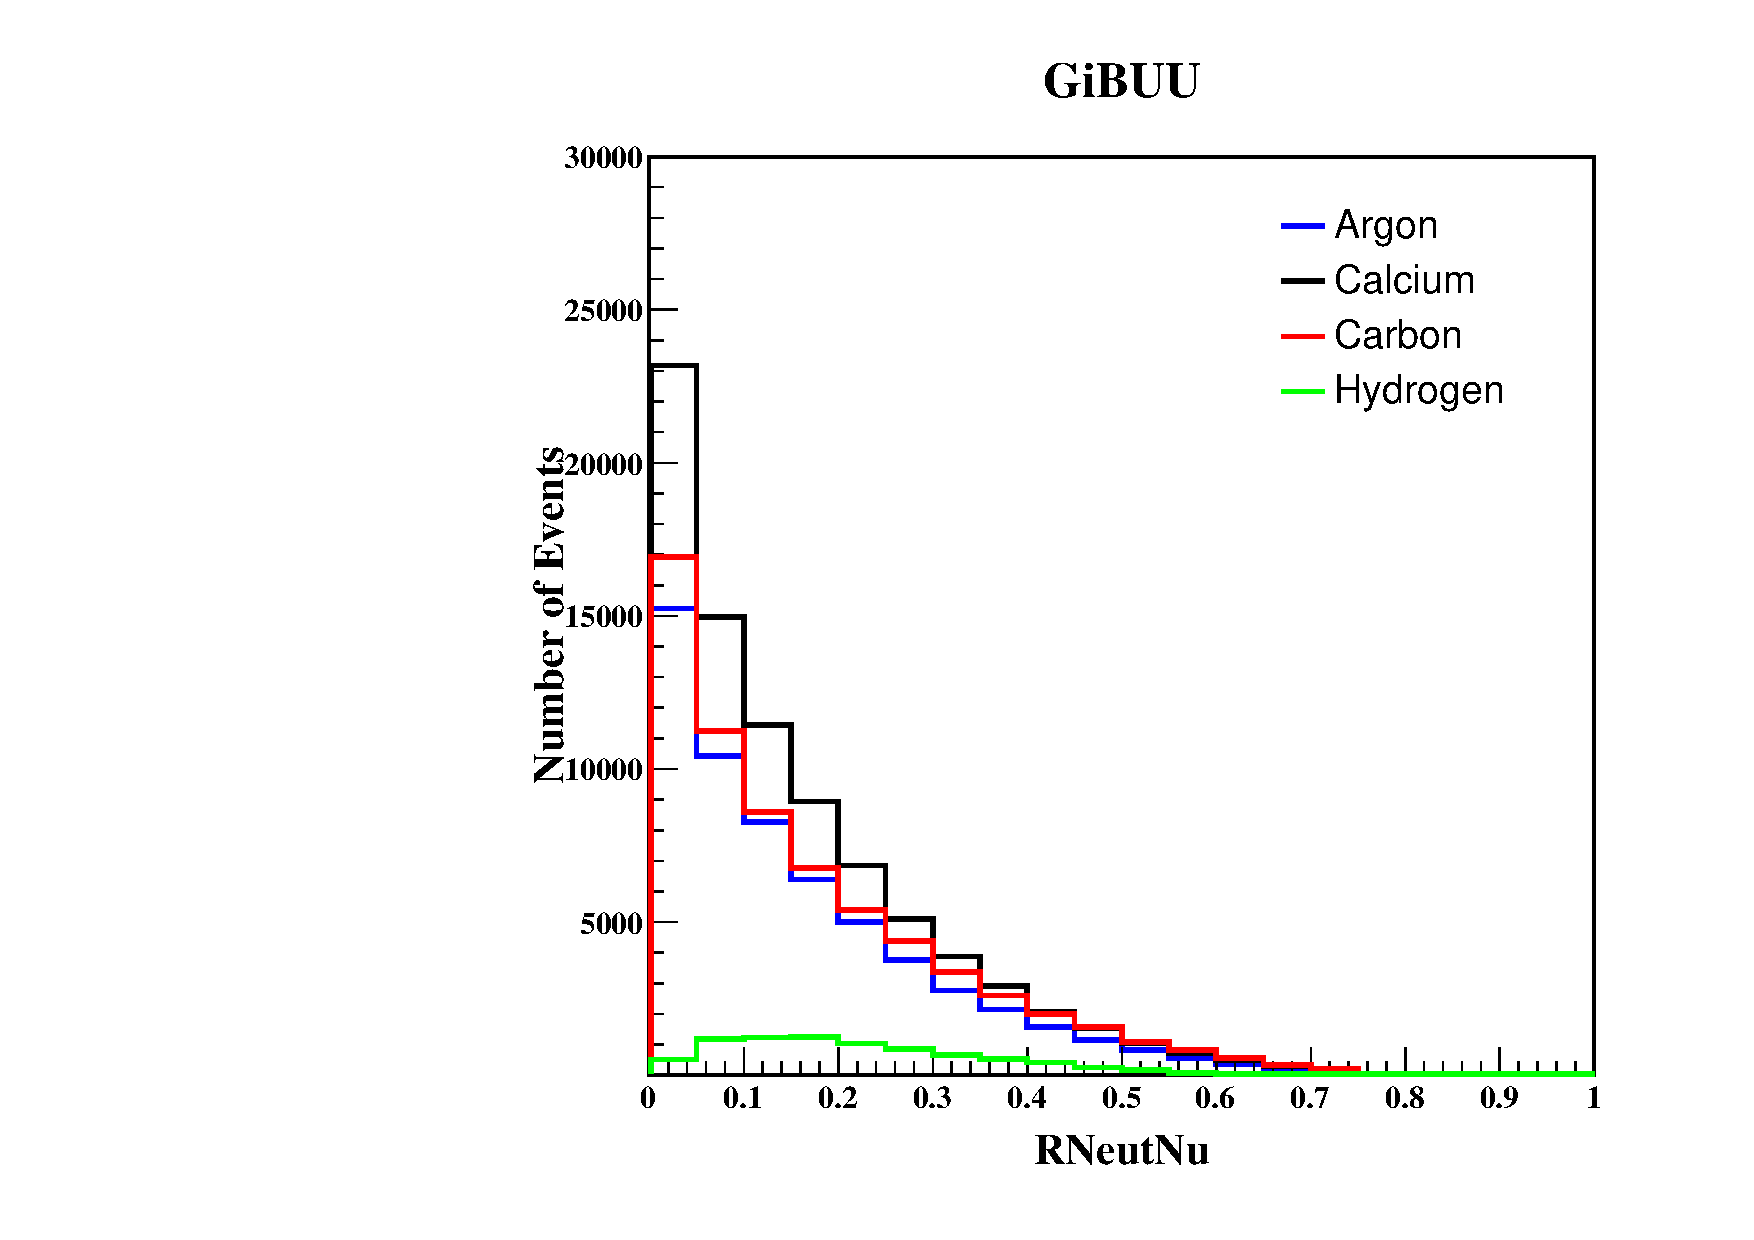
\includegraphics[scale=0.23]{Targets_25GeVRNeutNu}
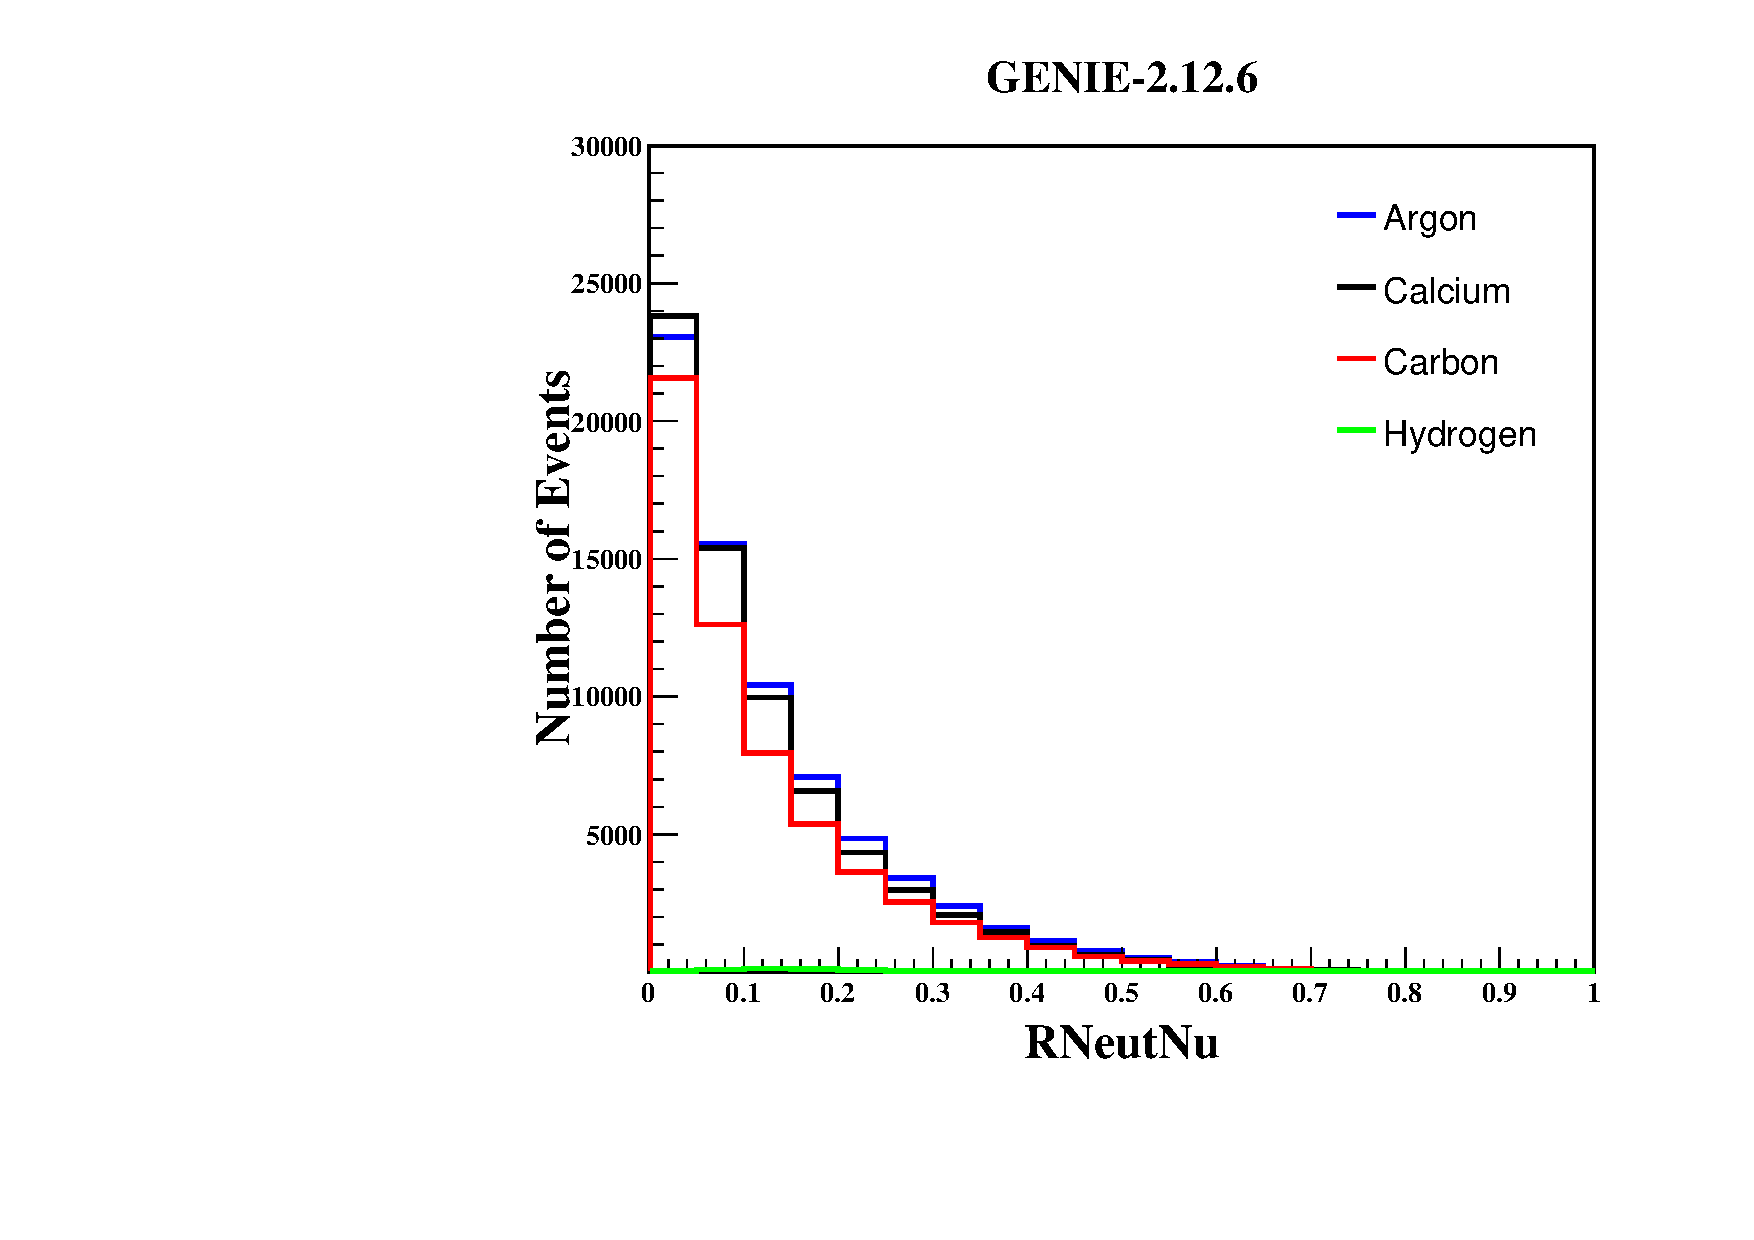
\includegraphics[scale=0.25]{AllTargetRNeutNu}
\end{figure}


\end{frame}

\begin{frame}
\begin{figure}
 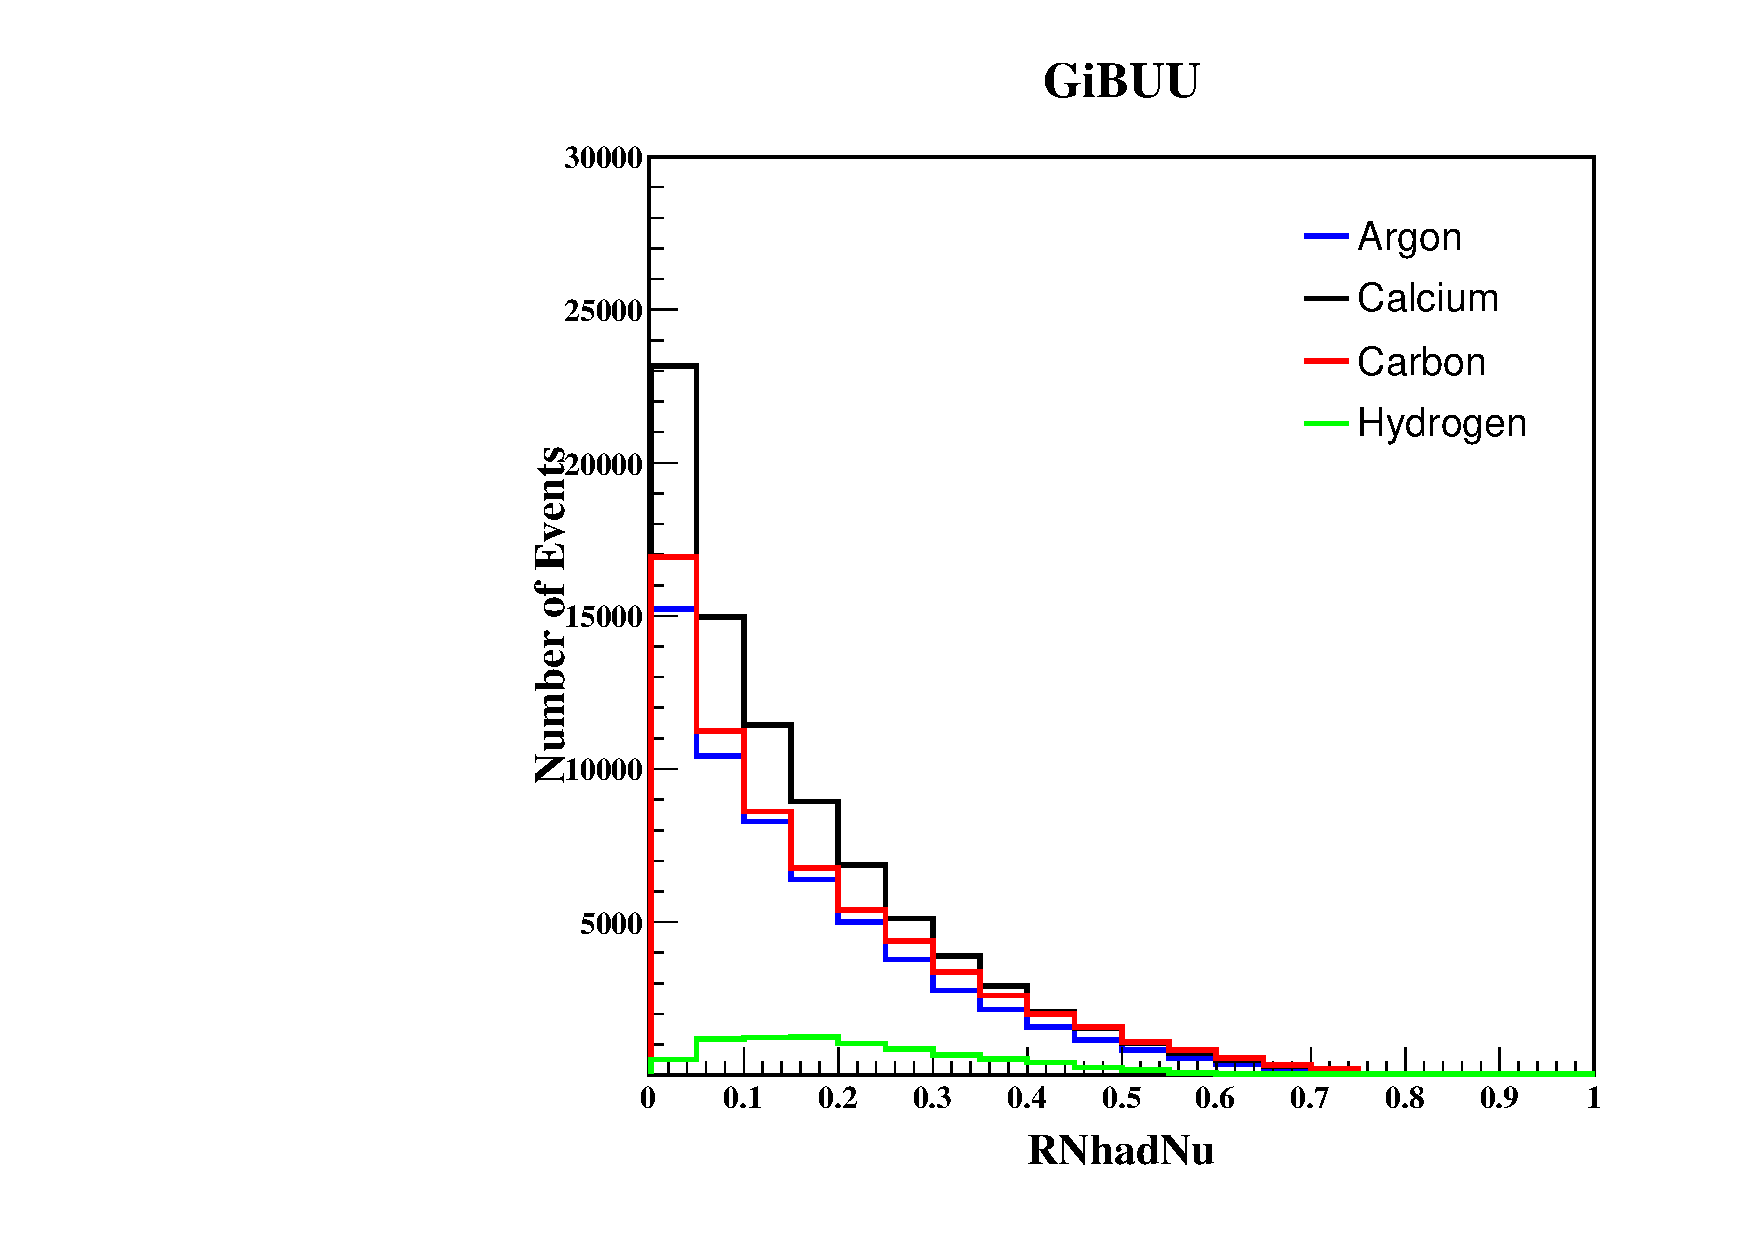
\includegraphics[scale=0.23]{AllTargetsRNhadNu}
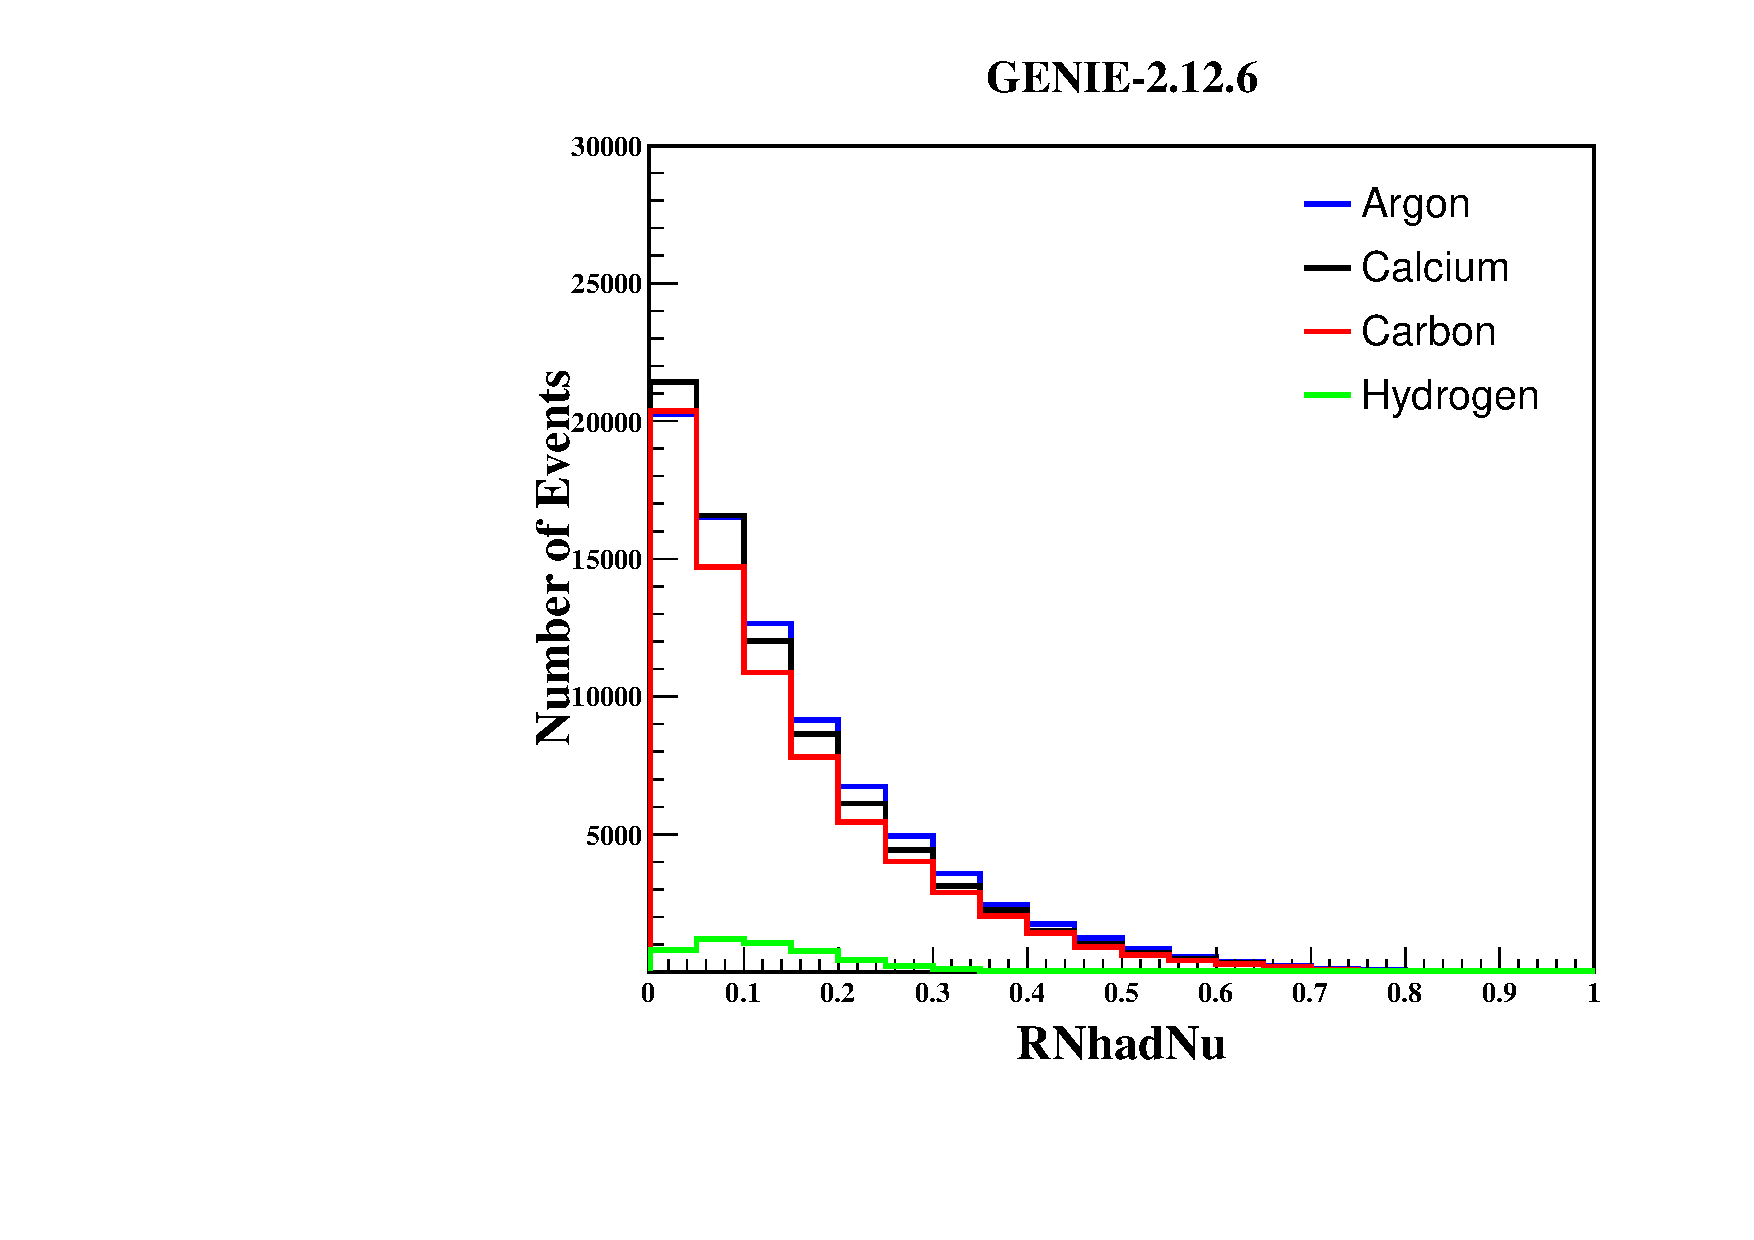
\includegraphics[scale=0.25]{AllTargetRNhadNu}

\end{figure}
\end{frame}




\end{document}
